\documentclass[a4paper,10pt]{article}
\usepackage[utf8x]{inputenc}
\usepackage{amsmath}
\usepackage{graphicx}
\usepackage{float}
\usepackage{hanging}
\usepackage[colorinitemizeoftodos]{todonotes}
\usepackage[lmargin=0.75in, rmargin=0.75in, top=1in, bottom=0.75in]{geometry}
\usepackage{lipsum}
\usepackage{multirow}
\usepackage{natbib}
\usepackage{cite}
\usepackage{listings}
\usepackage{multicol}



\usepackage{array}

\usepackage{color} %red, green, blue, yellow, cyan, magenta, black, white
\definecolor{mygreen}{RGB}{28,172,0} % color values Red, Green, Blue
\definecolor{mylilas}{RGB}{170,55,241}
\usepackage{graphicx}
\graphicspath{ {./images/} }
\usepackage{rotating}
\usepackage[section]{placeins}
\usepackage{tikz}
\usepackage[title]{appendix}
\usepackage[table,xcdraw]{xcolor}
\usepackage{setspace}
\usepackage{caption}
\graphicspath{ {./Images/} }
%Paragraph Style
\setlength\parindent{0pt}
\setlength{\parskip}{1em}


%TOC Formatting
\usepackage[subfigure]{tocloft}
\setlength\cftparskip{0pt}


%Section Header Formats
\usepackage{titlesec}
\titleformat{\section}
  {\normalfont\large\bfseries}{\thesection.}{0.5em}{}
\titleformat{\subsection}
  {\normalfont\normalsize\itshape}{\thesubsection.}{1em}{}
\titleformat{\subsubsection}
  {\normalfont\normalsize\itshape}{\thesubsubsection.}{1em}{}

\titlespacing{\section}{0}{0}{0}
\titlespacing{\subsection}{0}{0}{0}
\titlespacing{\subsubsection}{0}{0}{0}

%Multiple Images in One Figure Package
\usepackage{float}
\usepackage{subfigure}
%\usepackage{subcaption}
%\usepackage{amsmath}

% % code
% Better inline directory listings
\usepackage{listings}
\usepackage{xcolor}
\definecolor{light-gray}{gray}{0.95}
\newcommand{\code}[1]{\colorbox{light-gray}{\texttt{#1}}}
\definecolor{codegreen}{rgb}{0,0.6,0}
\definecolor{codegray}{rgb}{0.5,0.5,0.5}
\definecolor{codepurple}{rgb}{0.58,0,0.82}
\definecolor{backcolour}{rgb}{0.95,0.95,0.92}

\lstdefinestyle{mystyle}{
    backgroundcolor=\color{backcolour},   
    commentstyle=\color{codegreen},
    keywordstyle=\color{magenta},
    numberstyle=\tiny\color{codegray},
    stringstyle=\color{codepurple},
    basicstyle=\ttfamily\footnotesize,
    breakatwhitespace=false,         
    breaklines=true,                 
    captionpos=b,                    
    keepspaces=true,                 
    % numbers=left,                    
    % numbersep=5pt,                  
    showspaces=false,                
    showstringspaces=false,
    showtabs=false,                  
    tabsize=4
}

\lstset{style=mystyle}


%Page Headers
\usepackage{fancyhdr}
\pagestyle{fancy}
\fancyhf{}
\lhead{\nouppercase{\leftmark}}
\rhead{Nov 17, 2021}
\cfoot{\thepage}
\usepackage{hyperref}

\begin{document}
% \lstset{language=Matlab,%
%     %basicstyle=\color{red},
%     breaklines=true,%
%     morekeywords={matlab2tikz},
%     keywordstyle=\color{blue},%
%     morekeywords=[2]{1}, keywordstyle=[2]{\color{black}},
%     identifierstyle=\color{black},%
%     stringstyle=\color{mylilas},
%     commentstyle=\color{mygreen},%
%     showstringspaces=false,%without this there will be a symbol in the places where there is a space
%     numbers=left,%
%     numberstyle={\tiny \color{black}},% size of the numbers
%     numbersep=9pt, % this defines how far the numbers are from the text
%     emph=[1]{for,end,break},emphstyle=[1]\color{red}, %some words to emphasise
%     %emph=[2]{word1,word2}, emphstyle=[2]{style},    
% }
% %Citing by numbers
% \setcitestyle{numbers}

%%%%%%%%%%%%%%%%%%%%%%%%%%%%%%%%%%%%%%%%%%%%%%%%%%%%%%%%%%%%%%%%%%%%%%%%%%%%%%%%%%%%%%%%%%%%%%%%%%%%%%%%%%%%%%%%%%%%%%%%%%%%%%%%%%%%%%%%%%%%%%%%%%
\begin{titlepage}

\newcommand{\HRule}{\rule{\linewidth}{0.45mm}} % Defines a new command for the horizontal lines, change thickness here

\center % Center everything on the page
 
%	HEADING SECTIONS
\textsc{\LARGE Design with Embedding Operating Systems}\\[1.5cm] % Name of your university/college
\textsc{\Large Lab 401, Monday Section}\\[0.5cm] % Major heading such as course name
\textsc{\large }\\[0.5cm] % Minor heading such as course title

%	TITLE SECTION
\HRule \\[0.4cm]
{ \huge \bfseries Lab 4 Report}\\ % Title of your document
\HRule \\[0.5cm]

%	AUTHOR SECTION
\text{Sirena DePue | sgd63} \\
\text{Yu Zhang | yz2729} \\[6cm]

%   DATE SECTION
\text{November 17, 2021}\\




\vfill % Fill the rest of the page with whitespace

\end{titlepage}
%%%%%%%%%%%%%%%%%%%%%%%%%%%%%%%%%%%%%%%%%%%%%%%%%%%%%%%%%%%%%%%%%%%%%%%%%%%%%%%%%%%%%%%%%%%%%%%%%%%%%%%%%%%%%%%%%%%%%%%%%%%%%%%%%%%%%%%%%%%%%%%%%%

\tableofcontents

\newpage


\section{Introduction}

In this lab, we installed the PreemptRT kernel patch and explored the performance of a real-time operating system. In week 1, we performed some system measurements using cyclictest and perf to compare the startup latency and execution time (respectively) of a Python and C program. This was done under normal loading conditions and under high loading conditions, with all four cores being used. We then generated square waves using a Python and C script and compared the maximum frequency that is within 10\% of its nominal frequency. Then, we installed a new kernel, patched with PreemptRT by downloading the Linux source files and the patch, merging the patch with the Linux source, configuring the Linux code, compiling the Linux kernel, and finally copying the kernel to the SD card and booting the RPi. In week 2 we first ran through some configuration steps of the new kernel and patch. Then, we used the same techniques as in week 1 to measure the performance of the new system and compared the results.

As a note, we were not working together during week 1. Rather, Yu finished week 1 of lab on Monday, while Sirena was still checking off week 3 with her previous partner. We worked together the following week. 


\section{Design and Testing}

\subsection{Week 1}

\subsubsection{Part 1: Performance Measures}

\textbf{Performance Measure using Cyclictest}

For the first part of the lab, we determined the latency of the non-real-time operating system. The startup latency is measured using the tool \code{cyclictest}, which calls the process many times and records the startup latency for each instance in a histogram plot. Where latency varies between calls, the process is called many times to determine the range of latency and the average values of latency for each thread. Once this information is compiled, the deadline for a process can be set such that it encompasses part of the range to allow most processes to finish before their deadline. 

\code{cyclictest} is loaded and installed from github via the following commands:
\begin{center}
\begin{lstlisting}[language=bash, label=code:code1] 
git clone git://git.kernel.org/pub/scm/linux/kernel/git/clrkwllms/rt-tests.git
cd rt-tests
tmake all
sudo make install
sudo cyclictest --help
\end{lstlisting}
\end{center}\vspace{-1em}
% \quad \textit{git clone git://git.kernel.org/pub/scm/linux/kernel/git/clrkwllms/rt-tests.git}

% \quad \textit{cd rt-tests}

% \quad \textit{tmake all}

% \quad \textit{sudo make install}

% \quad \textit{sudo cyclictest --help}

We tested the installation via the command \code{cyclictest --help}. Then, we tested the execution of four threads running under low loading conditions (figure~\ref{Low Load on Original}) and the behavior of \code{cyclictest} while running cpu-intensive tasks (figure~\ref{High Load on Original}). The latter was achieved through a bash script that called \code{sort\_v1.c} about 20 times in the background. The \code{htop} command was uses to ensure the cores remained busy during the full duration of this test. The following command was used to check the latency of the system:
\begin{center}
\begin{lstlisting}[language=bash, label=code:code2] 
time sudo cylictest -p 90 -n -m -h 500 -t4 -l 300000
\end{lstlisting}
\end{center}\vspace{-1em}

% \quad \textit{time sudo cylictest -p 90 -n -m -h 500 -t4 -l 300000}

This runs four threads at priority = 90, uses the nanosleep timer, locks memory, records 500 histogram bins for 300000 loops. A summary of the minimum, average, and maximum latencies for the low and high CPU loads are shown below:

\begin{center}
\captionof{table}{Latency Ranges for Original Kernel [$\mu s$]}
\begin{tabular}{||c c c c||} 
 \hline
  & Min Range & Average Range & Maximum Range \\ [0.5ex] 
 \hline\hline
 Low Load & 6 & 13 & 472-580 \\ 
 \hline
 High Load & 7-8 & 25-34 & 1267-3069 \\ [1ex] 
 \hline
\end{tabular}
\end{center}

\begin{figure}[H]
\centering
\begin{minipage}{0.5\textwidth}
  \centering
  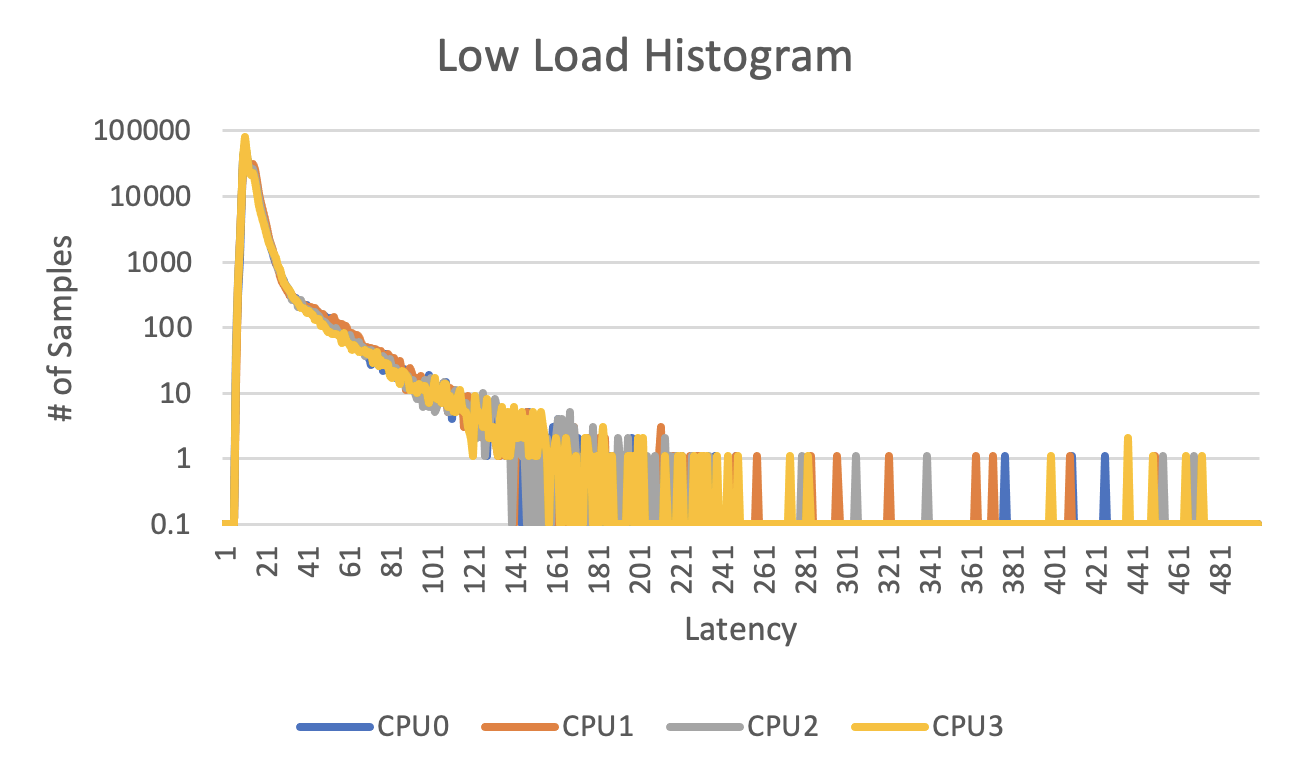
\includegraphics[width=1\linewidth]{Images/original - low load hist.png}
  \caption{Low Load on Original Kernel}
  \label{Low Load on Original}
\end{minipage}%
\begin{minipage}{0.5\textwidth}
  \centering
  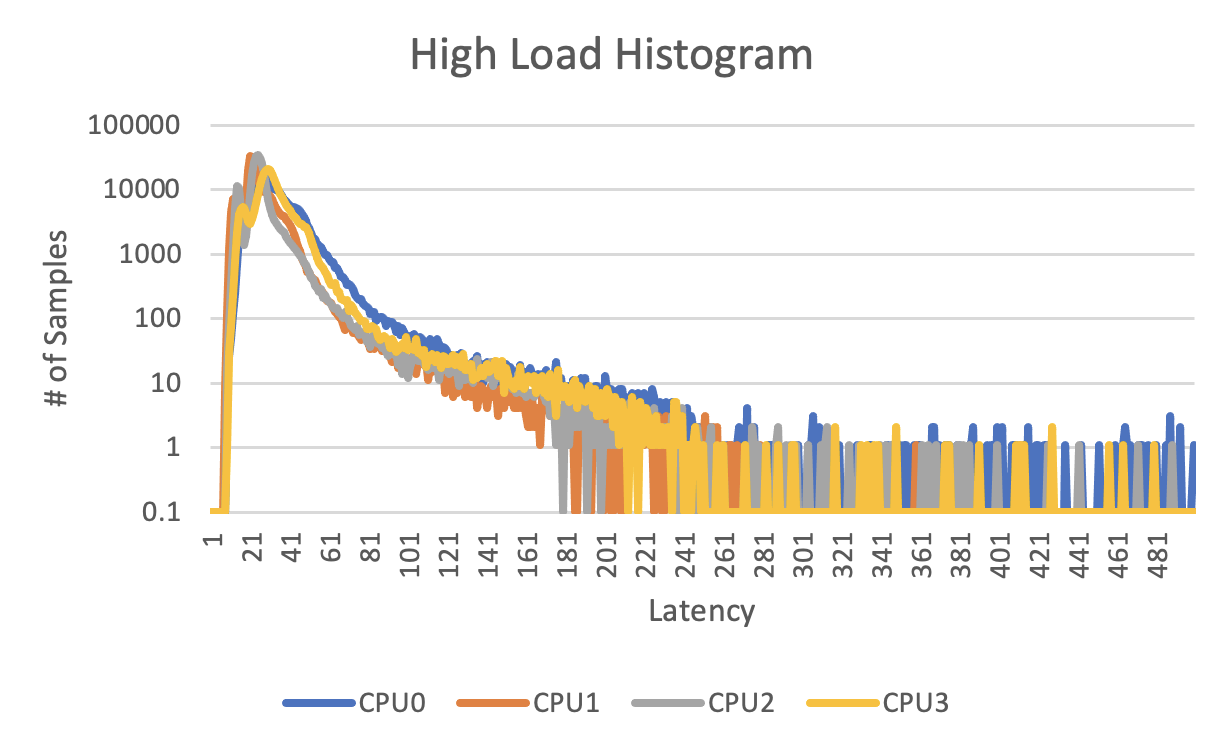
\includegraphics[width=1\linewidth]{Images/original - high load hist.png}
  \caption{High Load on Original Kernel}
  \label{High Load on Original}
\end{minipage}
\end{figure}

We can see that for the high CPU load, the minimum latency range is only slightly increased, while the average and maximum latency ranges increase significantly. The maximum latencies under high CPU load surpass the histogram plot, with latencies up to 3069 $\mu s$ (0.003069 s). The peak for low CPU load occurs in bin 10 at 80,792, meaning 10 $\mu s$ occurs the most frequently. The peak for high CPU load occurs in bin 30 at 33,856, meaning 30 $\mu s$ occurs the most frequently. There is a wide spread for both cases, with a higher variance in the high CPU load case. Overall, the high CPU load has greater variance and higher latency averages and maximums. It also shows a more gradual slope after the peak. 

A high CPU load reduces access to limited hardware resources and results in issues such as cache misses. These occur when a system makes a request to a cache for data, but the data is not in the cache memory. The system may then locate the data in the underlying data store and write the data to the cache, further increasing latency. Therefore, we would expect latency time to increase under high loading conditions.





\textbf{Performance Measure of sort.c using Perf}


Next, we use the tool \code{perf} to determine the execution time of \code{sort\_v1.c}. We downloaded this code from the ece5725-f21 server via:
\begin{center}
\begin{lstlisting}[language=bash, label=code:code3] 
/home/jfs9/lab4_files_f21/c_tests/sort_v1.c
\end{lstlisting}
\end{center}\vspace{-1em}
% \quad \textit{/home/jfs9/lab4\_files\_f21/c\_tests/sort\_v1.c}

Then, compiled the source via:
\begin{center}
\begin{lstlisting}[language=bash, label=code:code4] 
gcc -std=c99 -o sort_v1 sort_v1.c
\end{lstlisting}
\end{center}\vspace{-1em}

Finally, the call to perf was executed:
\begin{center}
\begin{lstlisting}[language=bash, label=code:code5] 
perf_4.18 stat ./sort_v1
\end{lstlisting}
\end{center}\vspace{-1em}

To display all recorded events, we logged into the ece5727\_f20 server, which runs a 5.4 linux kernel. After copying the approriate code, we were apply to compile and run it in the home directory. 

We ran the code for both sorted and unsorted cases and compared the outputs from perf (figures~\ref{Perf command unloaded} and~\ref{Perf command loaded}). The sorted script (sort the array prior to entering the loop to sum results) ran in about half the time and vastly reduces the number of branches missed. Therefore, sorting the data helps the CPU take the correct branch and saves clock cycles. A high CPU load load (via not sorting the data) reduces accuracy because the scheduler switches away from the script more frequently, so the timing and deadlines are less accurate. 

\begin{figure}[H]
\centering
\begin{minipage}{0.5\textwidth}
  \centering
  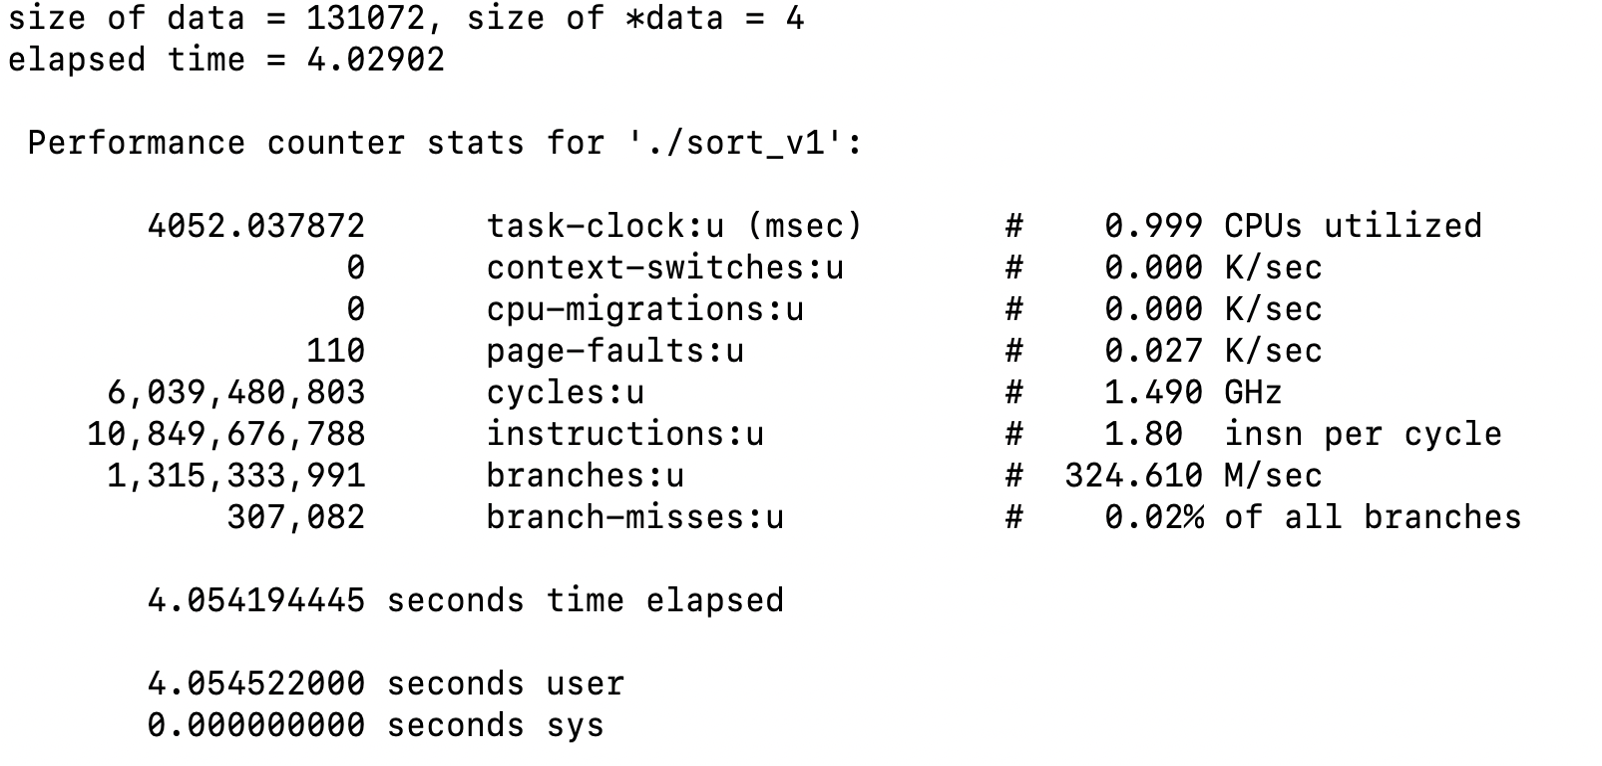
\includegraphics[width=0.9\linewidth]{Images/perf unloaded.png}
  \caption{Perf command on an unloaded system}
  \label{Perf command unloaded}
\end{minipage}%
\begin{minipage}{0.5\textwidth}
  \centering
  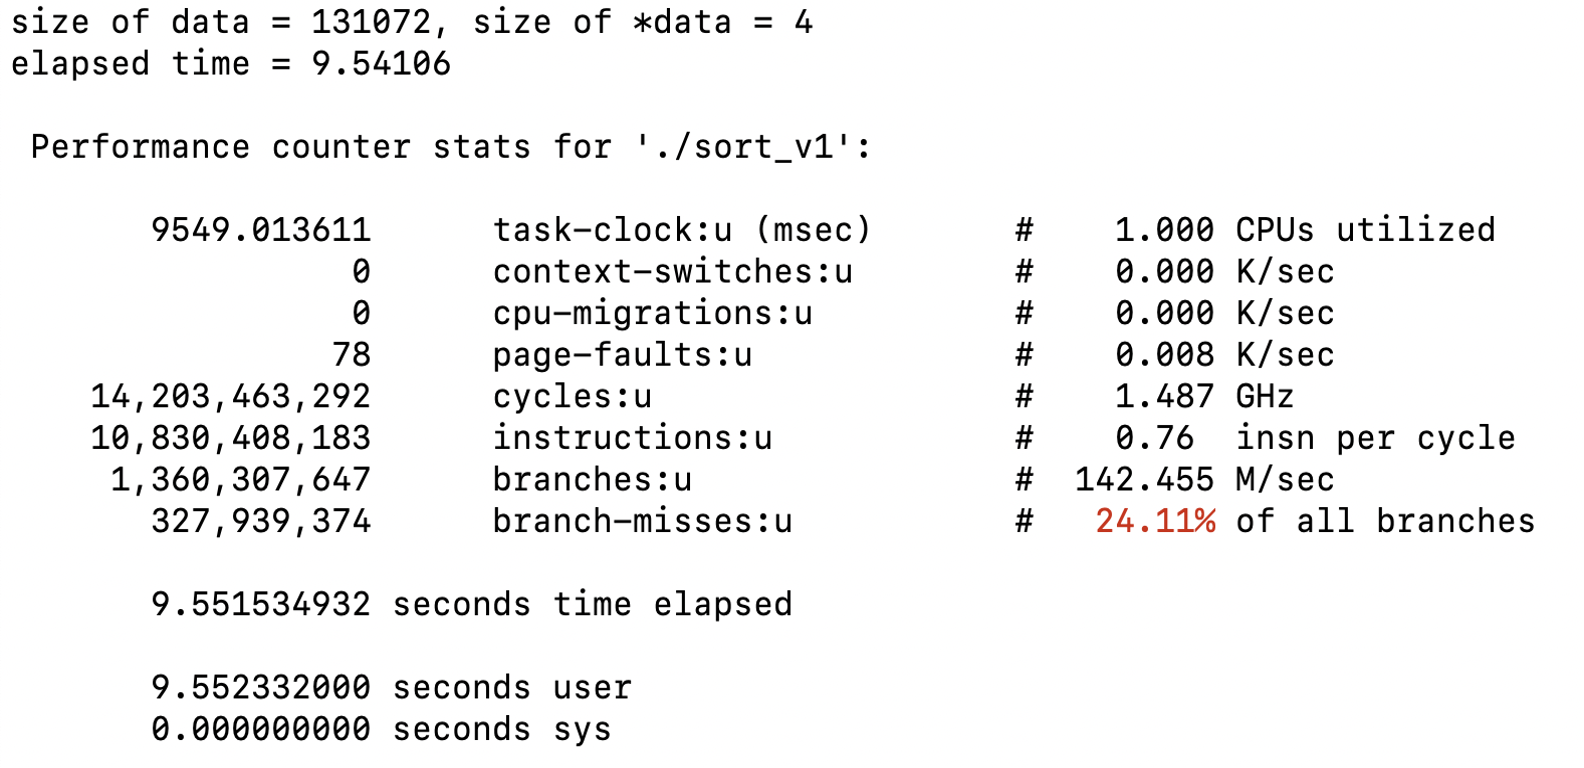
\includegraphics[width=0.9\linewidth]{Images/perf loaded.png}
  \caption{Perf command on a loaded system}
  \label{Perf command loaded}
\end{minipage}
\end{figure}

\textbf{Performance Measure of Square Wave in Python and C}

Finally, we generated square waves using a Python script \code{blink.py} and a C script \code{blink\_v7.c} and recorded the maximum frequency that is within 10\% of its nominal frequency. We used the oscilloscope since it displays the frequency, whereas PiScope requires the user to manually measure the frequency. The following command was used to compile the C code:
\begin{center}
\begin{lstlisting}[language=bash, label=code:code6] 
gcc -Wall -pthread -o blink_v7 blink_v7.c -lpigpio -lrt
\end{lstlisting}
\end{center}\vspace{-1em}
% \quad \textit{gcc -Wall –pthread -o blink\_v7 blink\_v7.c –lpigpio -lrt}

The circuit for this is as follows:

\begin{figure}[H]
\centering
\begin{minipage}{0.5\textwidth}
  \centering
  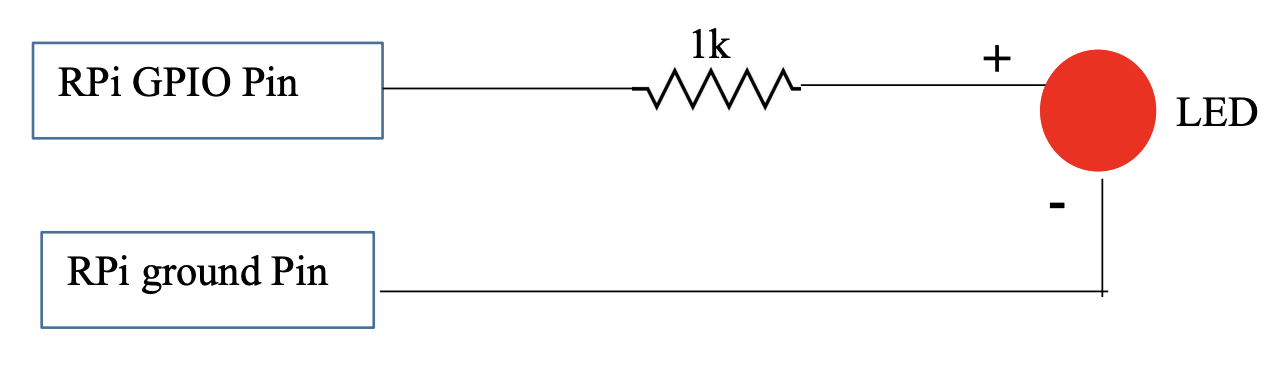
\includegraphics[width=0.9\linewidth]{Images/pinout diagram.png}
  \caption{Blink Pin-out Diagram}
\end{minipage}%
\begin{minipage}{0.5\textwidth}
  \centering
  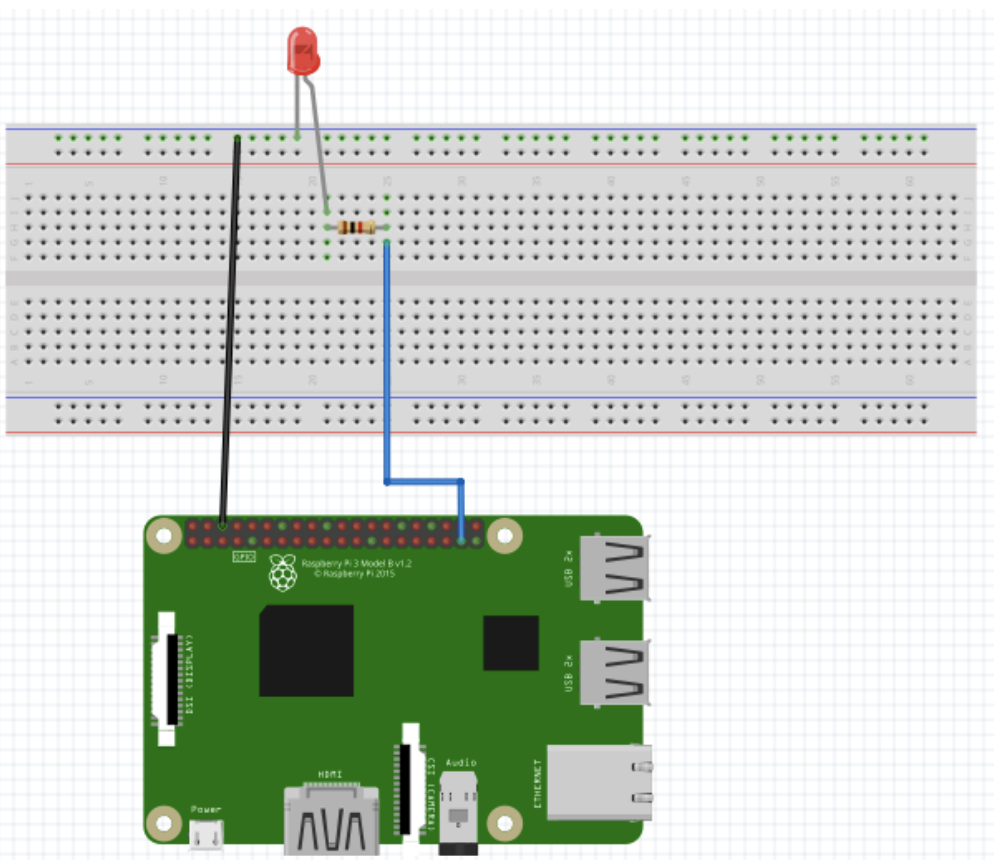
\includegraphics[width=0.9\linewidth]{Images/breadboard diagram.png}
  \caption{Blink Breadboard Diagram}
\end{minipage}
\end{figure}

The Python code results greatly differed from the C Code, which surprised us. Yu ran this on a 8 GB SD card, while Sirena ran this on a 16 GB SD card. This may have effected our differing results.

For the Python code, the maximum frequency for the unloaded system is almost the same as that of the loaded system. When Yu ran this, the value is around 1kHz, with the loaded system outperforming the unloaded system by 38 Hz (631 Hz vs 669 Hz).The screenshot of the oscilloscope are shown in the below figures. When we got this result, we thought for a moment that we had made a mistake in our testing methods as we believed that the maximum frequency should be higher for the unloaded system than for the loaded system. The professor and TA helped us to answer this question. Because Python is an interpreted language, it does not run very fast. Noise levels can effect our results and the load level of the system does not have a significant impact on the performance of the Python programs we tested.

\begin{figure}[H]
\centering
\begin{minipage}{0.5\textwidth}
  \centering
  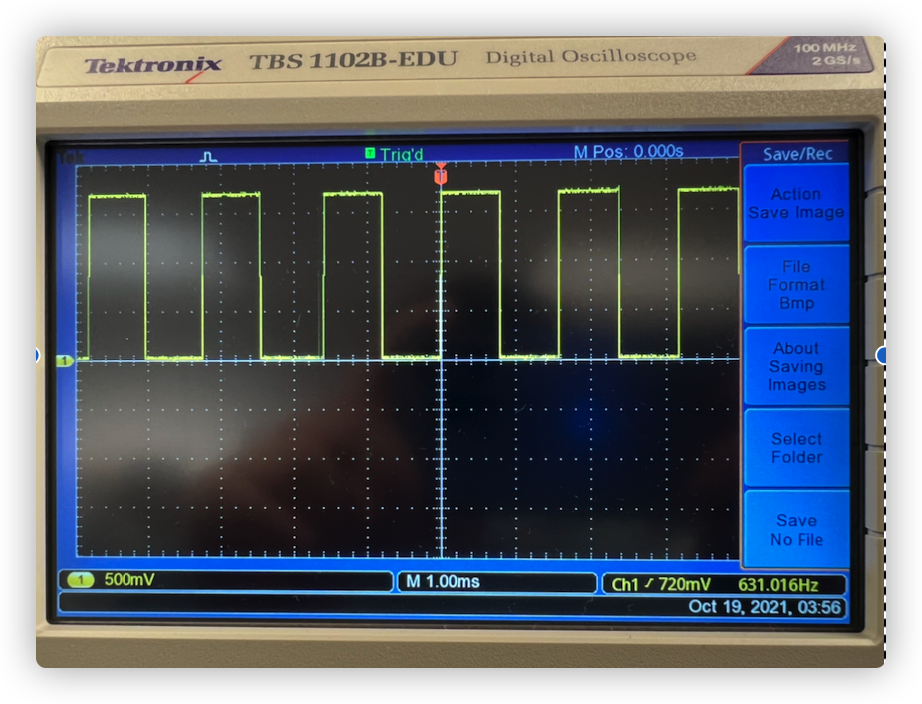
\includegraphics[width=\linewidth]{Images/python-loaded.png}
  \caption{Maximum frequency for loaded system}
\end{minipage}%
\begin{minipage}{0.5\textwidth}
  \centering
  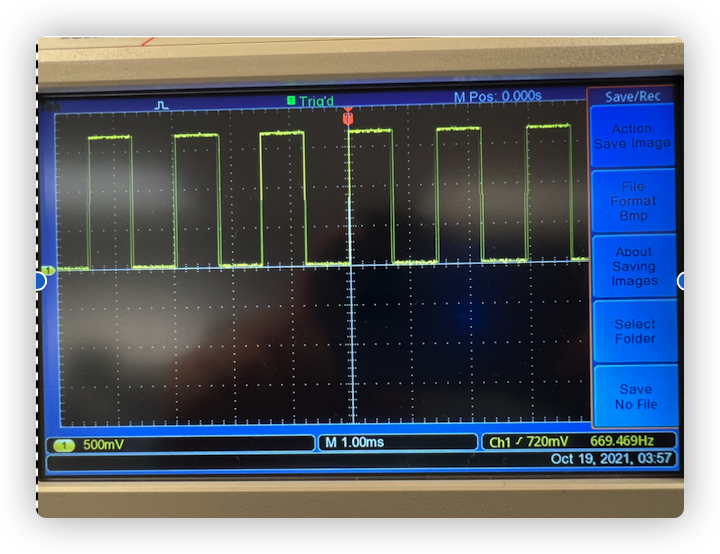
\includegraphics[width=\linewidth]{Images/pythonn-unloaded.png}
  \caption{Maximum frequency for unloaded system}
\end{minipage}
\end{figure}

When Sirena ran this, the value is also around 1 kHz, with the loaded system outperforming the unloaded system by 21 Hz (860 vs 881). However, we encountered a phenomenon that was quite strange when implementing higher frequencies. The maximum frequency for the Python code still maintained small difference between the loaded system and the unloaded system. However, the maximum value reaches about 5kHz. This was a very surprising result for us because we expected Python's maximum frequency would be around 1kHz. We tested the series of input frequency data twice, but the result did not change. This might just be due to some noise in Python and/or system overhead.

\begin{figure}[H]
\centering
  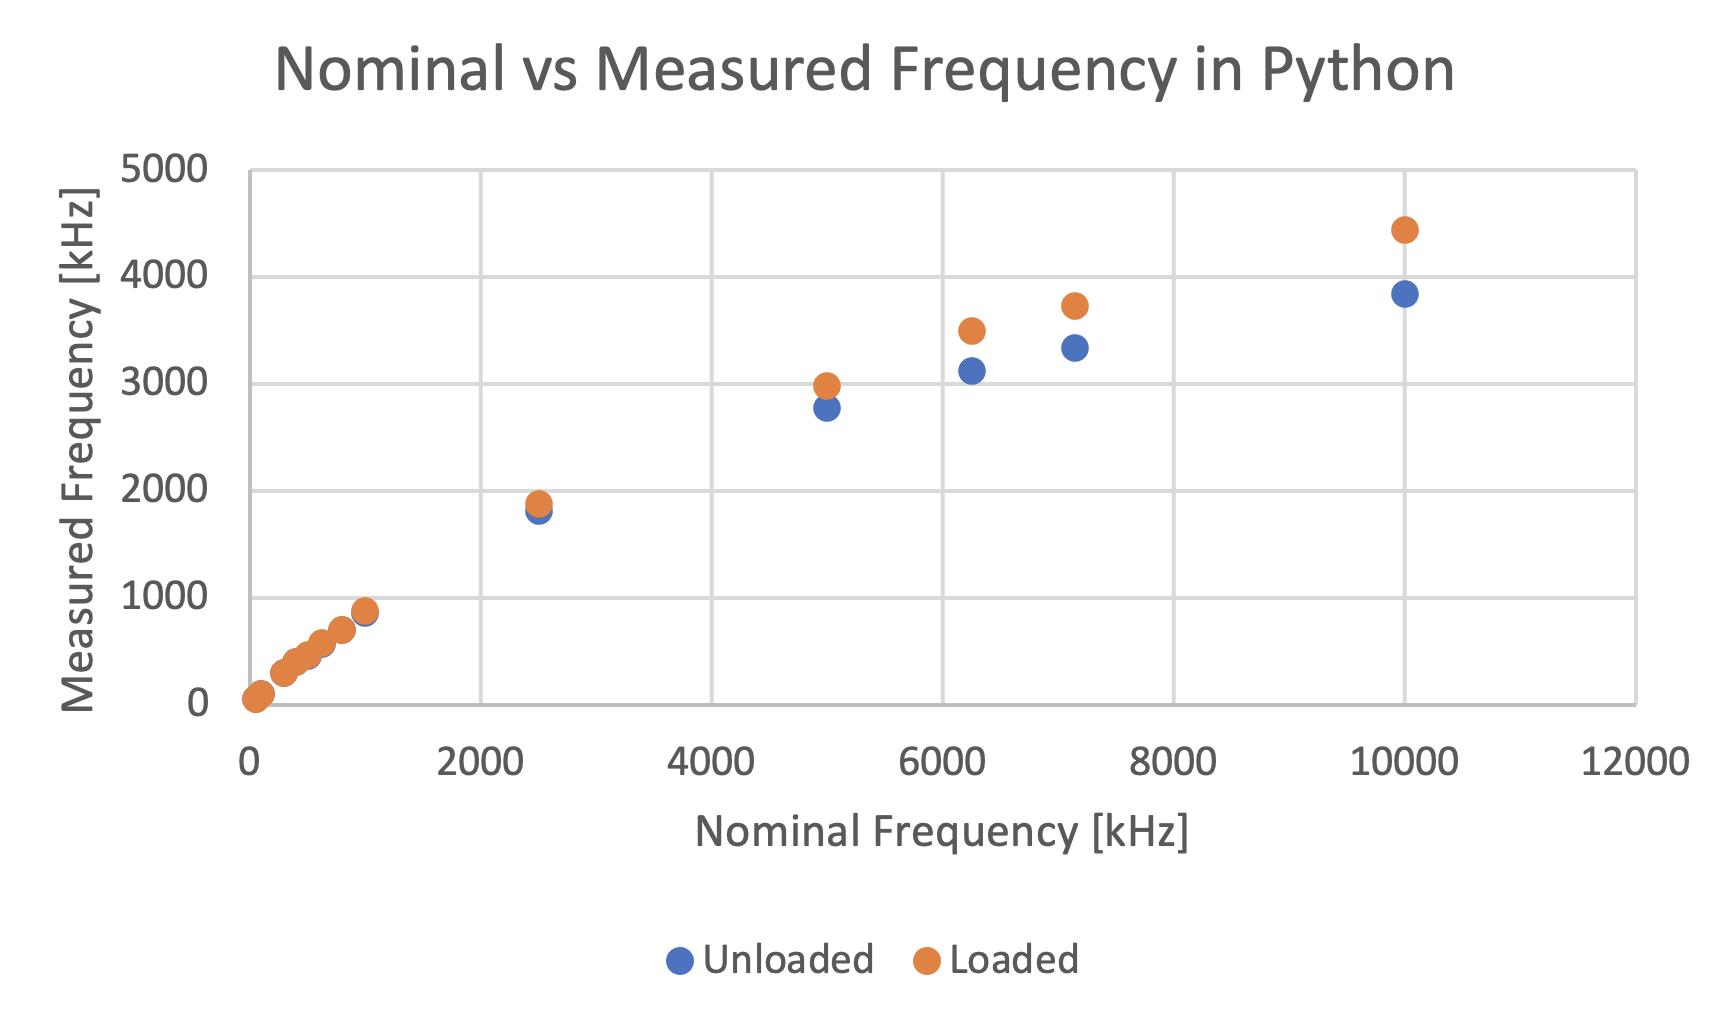
\includegraphics[width=0.75\linewidth]{Images/square wave python original.png}
  \caption{Blink Pin-out Diagram}
\end{figure}

The test results for C are very different from Python and match what we would have expected. The maximum frequency is about 50KHz for the unloaded system and 39KHz for the fully loaded system. These are significantly larger than the maximum frequencies of the Python code. Since Python is an interpreted language, whereas C is a compiled language, the execution time of Python will be slower because the number of CPU instructions required is much larger than that of machine code. The unloaded system outperforms the loaded system because high CPU load reduces accuracy. The scheduler switches away more frequently, so the timing and deadlines are less accurate. 

\begin{figure}[H]
\centering
  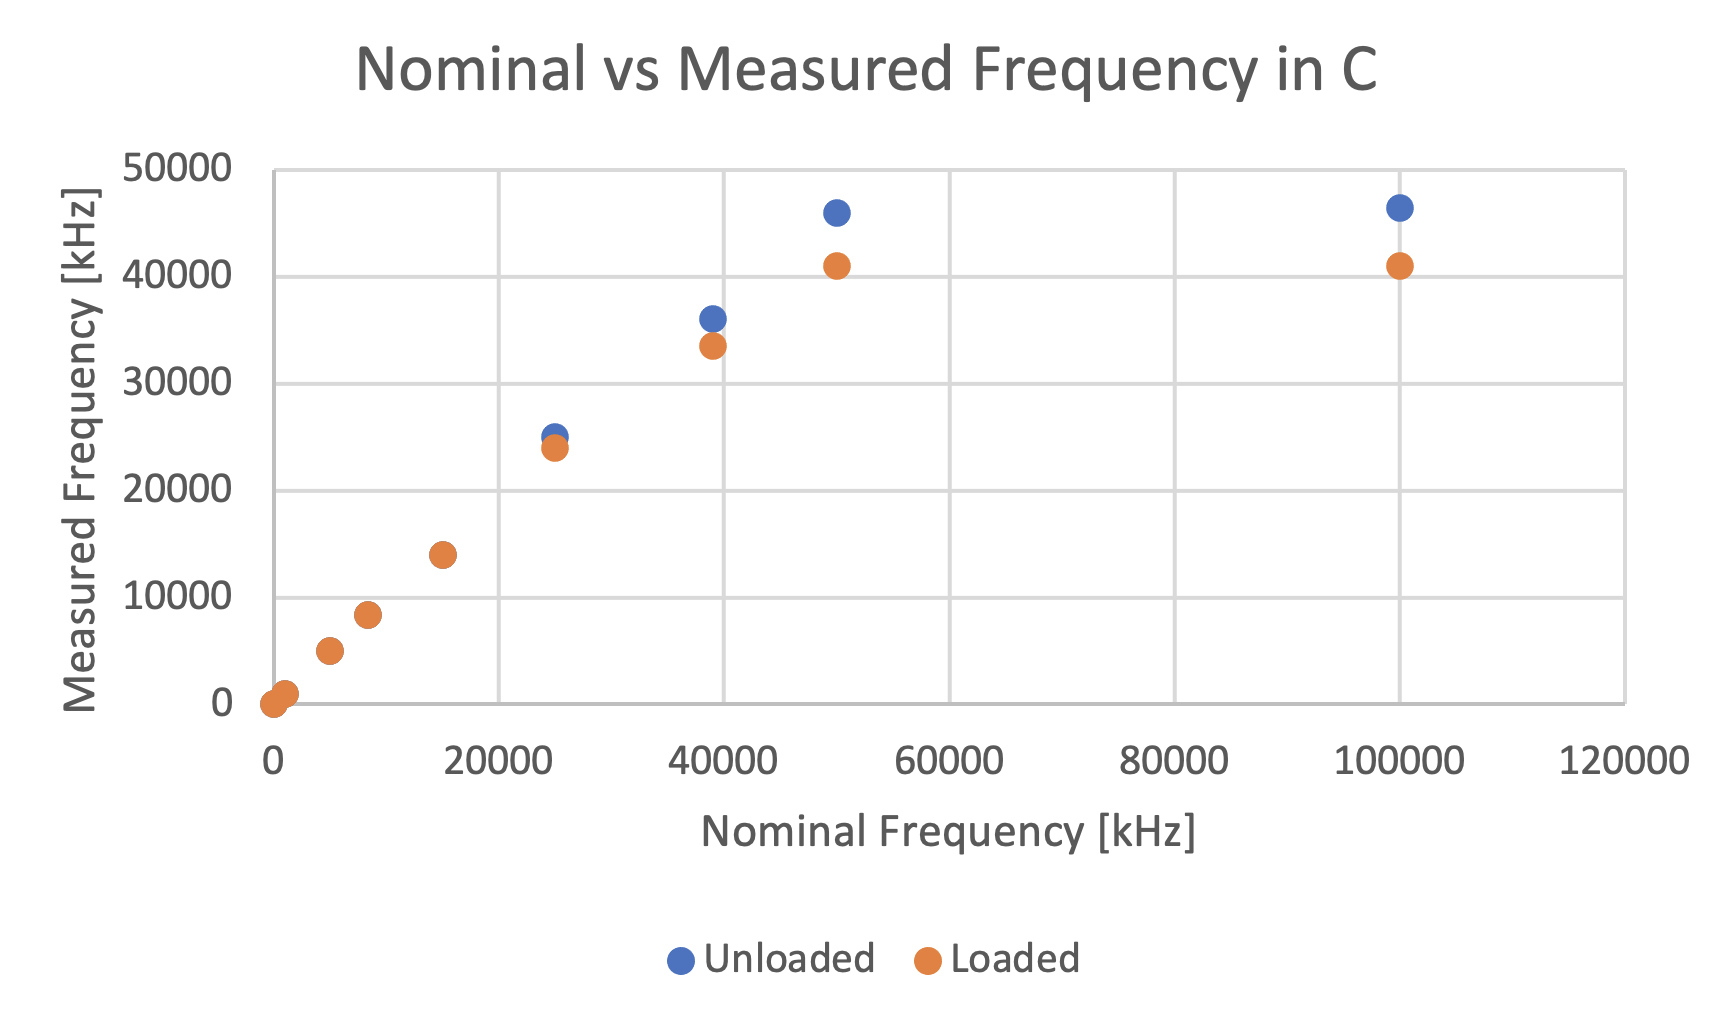
\includegraphics[width=0.75\linewidth]{Images/square wave c original.png} 
  \caption{Blink Pin-out Diagram}
\end{figure}

We encountered several issues when testing the C code. Initially, to meet the loading system requirements, Yu designed a program to calculate floating numbers and checked via \code{htop} that all 4 cores were occupied when the program ran. However, the maximum frequency (50KHZ) of the C program did not change between the unloaded system and the loaded system in this method. The professor suggested that the Raspberry Pi might have two sets of pipelines, one for floating  numbers and one for integers. Thus, the floating number program had no effect on the integer operations of our C program. We changed this method of loading the system to running \code{sort\_v1.c} 20 - 40 times at the same time in a bash script. So in summary, to successfully make the system fully loaded for the C program, not only do we need to make sure that 4 cores are fully occupied, but we also need to make sure that the loading program is of the integer type.

Finally, we learned how to easily test the maximum frequency. When our input frequency tends to infinity, the output frequency remains at the maximum frequency that the system can output. So, a simple way to test the maximum frequency is to directly input a very large frequency, for example 100MHZ, so that you can directly get the maximum evaluation frequency. This worked quite well to find an upper bound. 

% The results for the Python code is shown below in figure X. The maximum frequency is X for the unloaded system and X for the loaded system. 

% A similar phenomenon is seen for the C code in figure X. The maximum frequency is X for the unloaded system and X for the loaded system. 

\subsubsection{Part 2: Build the PreemptRT kernel}

We began with an SD card loaded with a copy of Raspbian from Lab3, and then compiled the 5.10.25 PreemptRT patch onto the RPi. This allows all the work to be done on the RPi platform, saves a few steps, and preserves the work done in Labs 1-3. However, the compile time is long (60 minutes) and requires the user to free space on the SD card before compilation. 

In addition to these processes documented below, we encountered two other problems. First, our SD card only had 8G, which was not enough to install PreemptRT. To resolve this, we simply migrated our system from an 8G SD card to a 16G SD card. Another issue is that \code{gcc} cannot be run successfully on our PreemptRT kernel system. This problem was caused by the system not recognising the original \code{gcc} version after installing PreemptRT. In order to fix this problem, we just reinstalled the \code{gcc} package via the following command:
\begin{center}
\begin{lstlisting}[language=bash, label=code:code17] 
sudo apt install gcc -t buster
\end{lstlisting}
\end{center}\vspace{-1em}

\textbf{Step 1: Initial Setup and Download Linux Source Files}

Start with you Lab 3 SD backup and remove any modifications to .bashrc so the kernel boots normally. Then, free space on the SD card via:

\begin{itemize}
    \item Remove large mp4 videos, games, and experimental applications 
    \item Remove wolfram-engine via \code{sudo apt-get remove --purge wolfram-engine} to free 2GB
    \item Remove supercollider via \code{sudo apt-get remove --purge supercollider*}
    \item Turn off swapping on in the current kernel
    \item Final set of commands to free 0.5GB: \code{sudo apt-get autoclean}, \code{sudo apt-get clean}, \\ \code{sudo apt-get autoremove}
\end{itemize}

To check the storage remaining, we issued the following commands:
\begin{itemize}
    \item \code{df -h} to check the free space in the filesystem
    \item \code{dpkg -get-selections} to show all installed applications
    \item \code{cd /INSERT\_DIRECTORY du -sh *} to detail the storage used in a particular directory
\end{itemize}

Next, load the appropriate C source code and clone the branch \code{rpi-5.10.y} to a local directory called 'linux' under the \code{/home/pi} directory to a depth of 700 (do not copy and paste):
\begin{center}
\begin{lstlisting}[language=bash, label=code:code7] 
cd /home/pi
time git clone --single-branch --branch 'rpi-5.10.y' --depth 700 https://github.com/raspberrypi/linux.git
\end{lstlisting}
\end{center}\vspace{-1em}
% \quad \textit{cd /home/pi}

% \quad time git clone --single-branch --branch ‘rpi-5.10.y’ –-depth 700
% https://github.com/raspberrypi/linux.git

Then, we checked the file system size via \code{df -h}. To check the version of the code downloaded, we ran \code{cd /home/pi/linux}, followed by \code{head Makefile} to indicate the level downloaded. To switch to the 5.10.25 source level, we ran \code{git checkout 3e55254ce6f792372bbfe90f77006e75467c1dfe} to repoint the source branch to the last known commit for the 5.10.25 Linux source branch. To check this worked, we reran the \code{cd /home/pi/linux} and \code{head Makefile} commands to ensure the release level is 5.10.25. 

Next, we install missing dependencies by running:
\begin{center}
\begin{lstlisting}[language=bash, label=code:code8] 
sudo apt install bc bison flex
sudo apt install libncurses5-dev -t buster
sudo apt install libssl-dev -t buster
\end{lstlisting}
\end{center}\vspace{-1em}
% \quad \textit{sudo apt install bc bison flex}

% \quad \textit{sudo apt install libncurses5-dev -t buster}

% \quad \textit{sudo apt install libssl-dev –t buster}

\textbf{Step 2: Download the PreemptRT Patch and Merge with Kernel Source}

Copy the PreemptRT-patch directly into the linux source directory via:
\begin{center}
\begin{lstlisting}[language=bash, label=code:code9] 
cd /home/pi/linux
wget https://www.kernel.org/pub/linux/kernel/projects/rt/5.10/older/patch
-5.10.25-rt35.patch.gz
\end{lstlisting}
\end{center}\vspace{-1em}

% \quad \textit{cd /home/pi/linux}

% \quad \textit{wget
% https://www.kernel.org/pub/linux/kernel/projects/rt/5.10/older/patch -5.10.25-rt35.patch.gz}
Then, backup the SD card and apply the following patches to the linux source:
\begin{center}
\begin{lstlisting}[language=bash, label=code:code10] 
cd /home/pi/linux
zcat patch-5.10.25-rt35.patch.gz | patch -p1 > /home/pi/patch.log 2>&1
\end{lstlisting}
\end{center}\vspace{-1em}

% \quad \textit{cd /home/pi/linux}

% \quad \textit{zcat patch-5.10.25-rt35.patch.gz | patch -p1 > /home/pi/patch.log 2>&1}

Check \code{/home/pi/patch.log} to make sure there are no errors. 

\textbf{Step 3: Configure the Kernel}

Begin by ensuring the install will begin with a clean make environment by removing an previously compiled files from the \code{/linux} directory via \code{make clean} and \code{make mrproper}. Give the kernel image the correct name (kernel71):
\begin{center}
\begin{lstlisting}[language=bash, label=code:code11] 
KERNEL=kernel7l # Setting to compile the RPi 4 kernel
echo \$KERNEL # to check environment variable setting
kernel7l # kernel7 will be returned if setting is correct
make bcm2711_defconfig  # use make to build the RPi4 config file
\end{lstlisting}
\end{center}\vspace{-1em}
% \quad \textit{KERNEL=kernel7l} \# Setting to compile the RPi 4 kernel

% \quad \textit{echo \$KERNEL} \# to check environment variable setting

% \quad \textit{kernel7l} \# kernel7 will be returned if setting is correct

% \quad \textit{make bcm2711\_defconfig} \# use make to build the RPi4 config file

Run \code{make menuconfig} to check and change settings for the upcoming application: 

\begin{itemize}
    \item In 'General Setup', 'preemption model, select 'RT Fully Preemptable kernel'. 
    \item In 'General Setup', 'Timers subsystem', select High Resolution Timer Support'
    \item Save changes and exit
\end{itemize}

\textbf{Step 4: Compile the Patched, Configured Kernel}

First, check the free space on the card via \code{df -h} - it should have at least 5GB free. Then, check the value of the \code{\$KERNEL} environment variable (see above). To compile (60 min), we ran the following commands:
\begin{center}
\begin{lstlisting}[language=bash, label=code:code12] 
date # a time reference for when the compilation begins
time make -j4 zImage modules dtbs $>$ /home/pi/make.log 2$>$\&1
\end{lstlisting}
\end{center}\vspace{-1em}

% \quad \textit{date} \# a time reference for when the compilation begins

% \quad \textit{time make –j4 zImage modules dtbs $>$ /home/pi/make.log 2$>$\&1}

In a second window:
\begin{center}
\begin{lstlisting}[language=bash, label=code:code13] 
tail -f make.log # to watch progress
\end{lstlisting}
\end{center}\vspace{-1em}
% \quad \textit{tail –f make.log} \# to watch progress

Once compiled, we checked for warnings or errors in make.log and compared it to the sample \code{make.log} saved in \code{/home/jfs9/lab4\_files\_f21} on the class
server. We also checked to ensure the \code{\$KERNEL} environment variable was still set. Then we issued the command: \code{time sudo make –j4 modules\_install $>$ /home/pi/modules\_ins}\\\code{tall.log 2$>$\&1} to start four tasks to use all four processors. 

Finally, we backed up the SD card.

We both finished before the next week, with Yu finishing in Monday's lab and Sirena finishing in subsequent office hours.
 

\subsection{Week 2}

A non real-time system cannot be expressed as a function of time and results in longer deadlines. On the other hand, real-time systems have an associated time bound that can be expressed quantitatively as a function of time. This is separated into two categories: hard real time system and soft real time system. A hard real time system is very restrictive in that it strictly enforces deadlines and classifies a missed deadline as a system failure. A soft real time system is less restrictive and allows missed deadlines as long as processes are still executed in a timely manner. Where real-time systems result in lower latency times, they would typically be used in the case of mission critical applications.


\subsubsection{Step 1: Set up the PreemptRT kernel}
Before we can start our week2 test experiments, there are a few more steps to complete to get the PreemptRT kernel set up.

After completing compilation and backup the SD card. Once the SD card is backed up, reboot and continue with the remaining installation steps.

Run the command \code{uname -a} and record the results to confirm the updated kernel version - 5.10.63. Our results are shown below:

\begin{figure}[H]
\centering
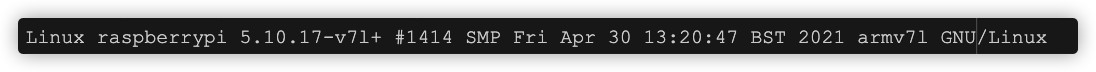
\includegraphics[width=0.75\linewidth]{Images/uname1.png}
\caption{Kernel Version before new kernel installation}
\end{figure}

Use the following commands to set the \code{\$KERNEL} environment variable:
\begin{center}
\begin{lstlisting}[language=bash, label=code:code14] 
cd /home/pi/linux # linux source directory
KERNEL=kernel171 # set the KERNEL environment variable
\end{lstlisting}
\end{center}\vspace{-1em}

% \quad cd /home/pi/linux \textit{\# linux source directory}

% \quad KERNEL=kernel171 \textit{\# set the KERNEL environment variable}

Now use the following commands to move compiled results in the \code{/linux} directory to the \code{/boot} location of the current Linux kernel:

\begin{center}
\begin{lstlisting}[language=bash, label=code:code15] 
echo \$KERNEL  # check KERNEL setting - desired return is "kernel171"
sudo cp arch/arm/boot/dts/*.dtb /boot/
sudo cp arch/arm/boot/dts/overlays/*.dtb* /boot/overlays/
sudo cp arch/arm/boot/dts/overlays/README /boot/overlays/
sudo cp arch/arm/boot/zImage /boot/\$KERNEL.img
\end{lstlisting}
\end{center}\vspace{-1em}

After these commands are run, reboot to start the PreemptRT kernel. Then, run the command \code{uname -a} and we can get the result shown in bellow which demonstrate that we already run the system with the PreemptRT kernel.
\begin{figure}[H]
\centering
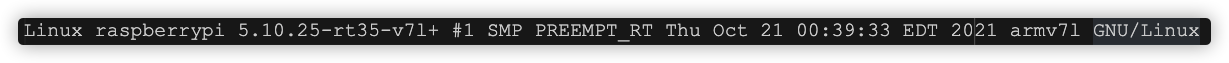
\includegraphics[width=\linewidth]{Images/uname2.png}
\caption{Kernel Version after new kernel installation}
\end{figure}

One last configuration step is to add a line in the file \code{/boot/cmdline.txt}. The content is shown below:
\begin{center}
\begin{lstlisting}[language=bash, label=code:code15] 
dwc_otg.fig_enable=0 dwc_otg.fig_fsm_enable=0 dwc_otg.nak_holdoff=0
\end{lstlisting}
\end{center}\vspace{-1em}

Finally, we can reboot the system and then backup the SD card. All the configuration steps have been done at this point.

\subsubsection{Step 2: Check Performance of the PreemptRT System}
In this section, we will show our test results of the PreemptRT system. There are three performance measure tests and they will be described below.

\textbf{Step 1: Cyclictest Result}

To perform the \code{cyclictest}, we need to run the command \code{udo cyclictest -p 90 -n –m -h 500 -t4 -l 300000} in the unloaded system and the loaded system.

A summary of the minimum, average, and maximum latencies for the low and high CPU loads are shown below:

\begin{center}
\captionof{table}{Latency Ranges for PreemptRT Kernel [$\mu s$]}
\begin{tabular}{||c c c c||} 
 \hline
  & Min Range & Average Range & Maximum Range \\ [0.5ex] 
 \hline\hline
 Low Load & 7 & 14-15 & 87-123 \\ 
 \hline
 High Load & 7 & 12-15 & 80-99 \\ [1ex] 
 \hline
\end{tabular}
\end{center}

In the PreempRT kernel, we see low average and maximum latencies ranges, even under high CPU load.
We can see that for the high CPU load, the minimum latency remains the same, while the average and maximum latency range slightly decreases. The peak for the low CPU load occurs in bin 9 at 53,871, meaning a latency of 9 $\mu s$ occurs the most frequently. The peak for the high CPU load occurs in bin 10 at 77,433, meaning a latency of 10 $\mu s$ occurs the most frequently. This marks a 10.5\% difference is the global maximas. In both instances, the variance for both are quite small. For low CPU load, the largest latency is 123 $\mu s$, which only occurs once. For the high CPU load, the largest latency is 99 $\mu s$, which only occurs once.  Under low and high load CPU, the distributions of the histogram are similar and both have short tails. Under high load, the histogram plateaus briefly near 45 $\mu s$, which might explain why the average range has a lower minimum value than under low loading conditions. Overall, there is no significant differences between latency times under low and high CPU load, contrary to the original kernel. 

\begin{figure}[H]
\centering
\begin{minipage}{0.5\textwidth}
  \centering
  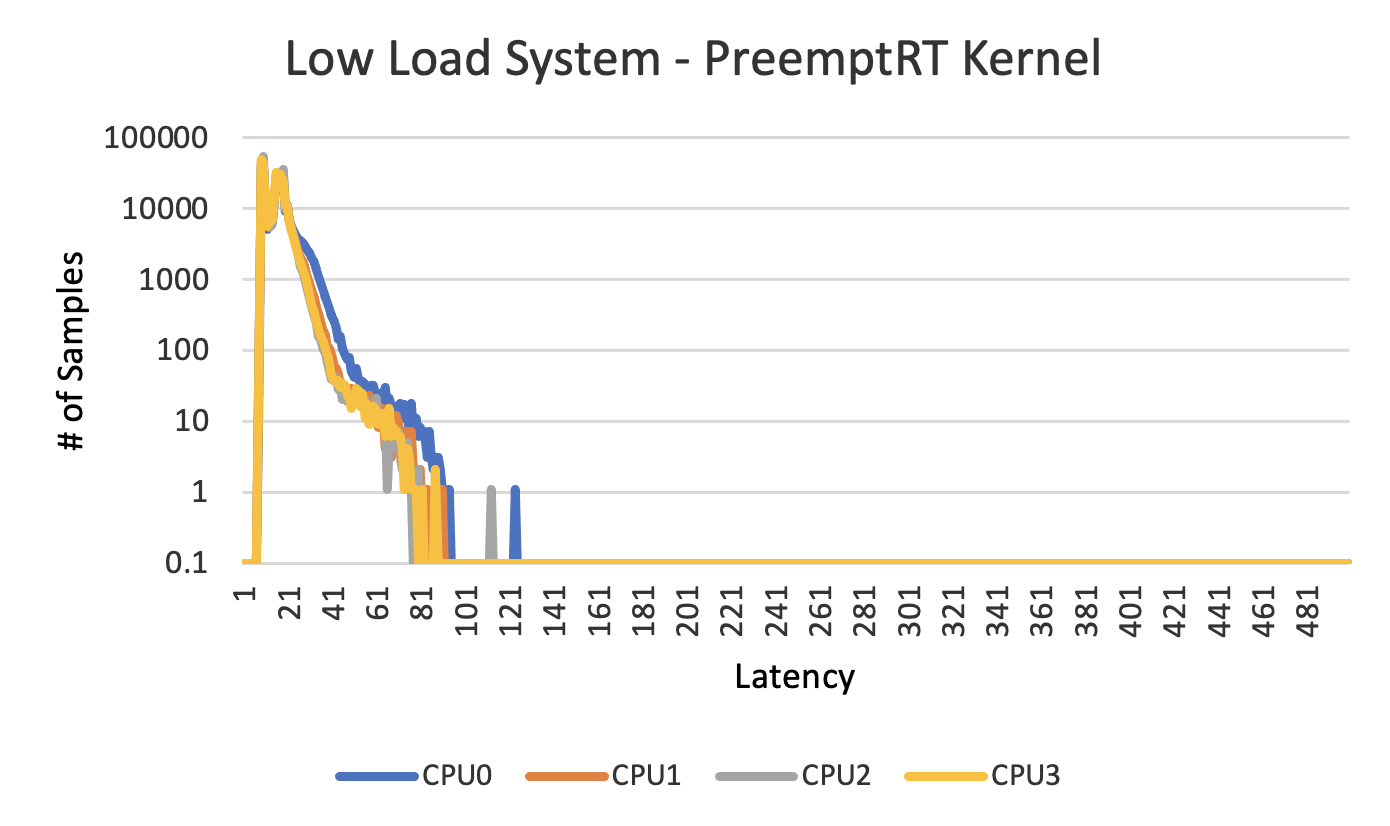
\includegraphics[width=0.9\linewidth]{Images/preempt - low load hist.png}
  \caption{Low Load on Preempt Kernel}
\end{minipage}%
\begin{minipage}{0.5\textwidth}
  \centering
  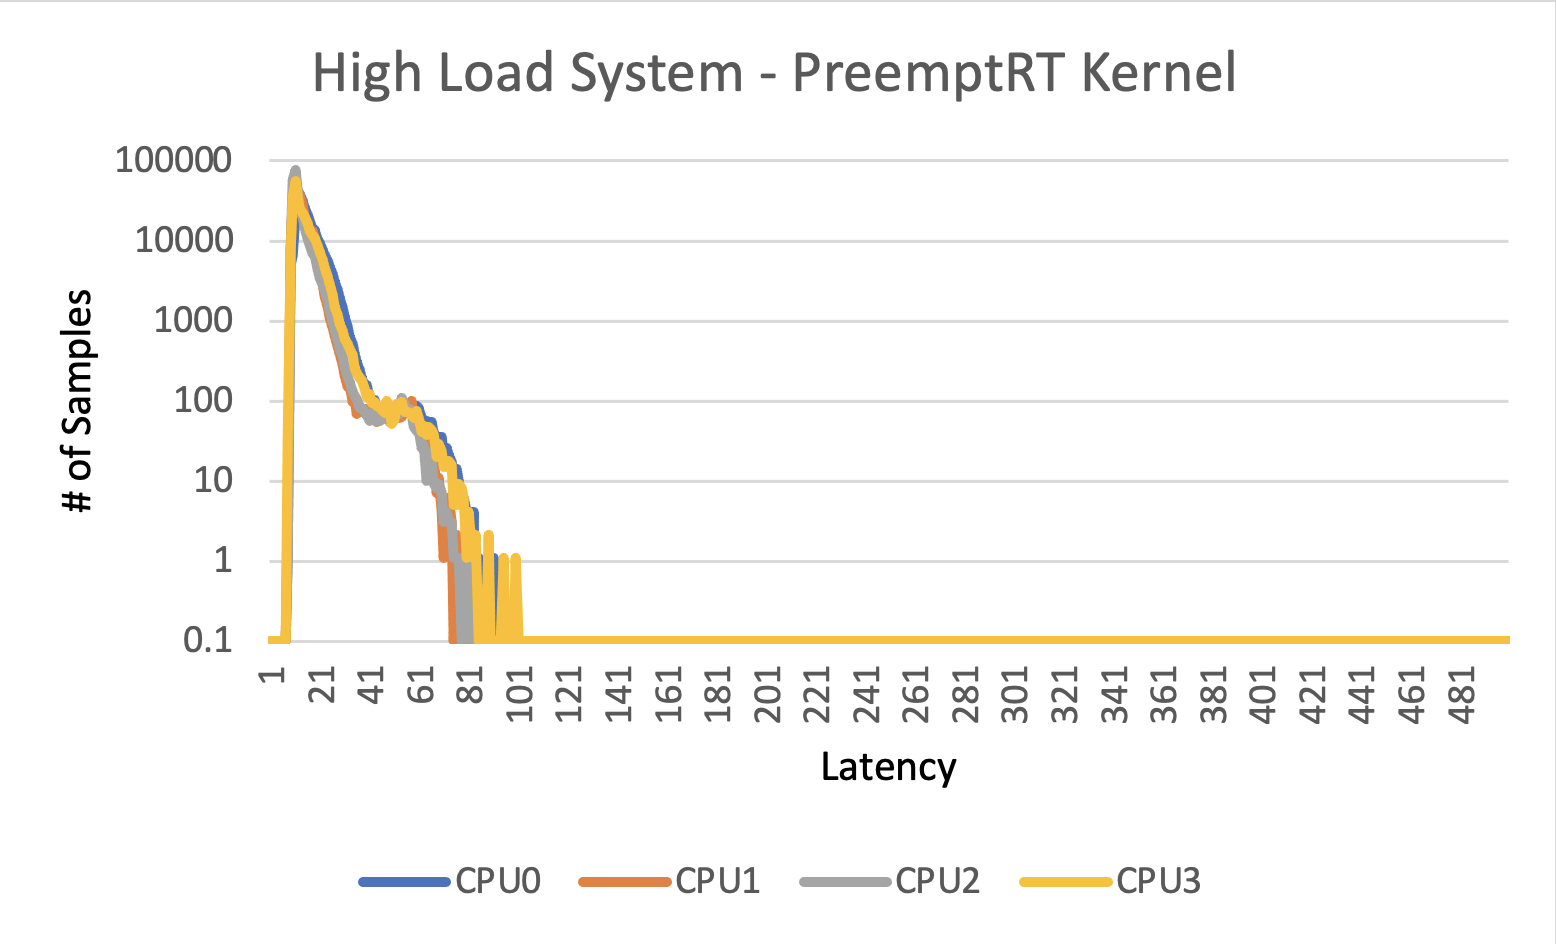
\includegraphics[width=0.9\linewidth]{Images/preempt - high load hist.png}
  \caption{High Load on Preempt Kernel}
\end{minipage}
\end{figure}

When considering the histograms from the loaded and unloaded original kernel, this marks a clear reduction in the maximum latency of the system and shows significantly less variation. We can see the maximum latency for the loaded system is much smaller, which explains the higher average scheduling latency in the original kernel under high loading. Despite the maximum latency for the unloaded system also being much smaller, the average range is slightly higher than that of the original kernel. This is likely due to the distribution of the histogram; it steeply drops after reaching its global maxima in the original kernel histogram. The narrower histograms demonstrate improved scheduling and allowing tasks to execute before context switching. 

The table below shows the percent differences between the maximum of the minimum, average, and maximum range. The negative values indicate a reduction in latency while positive values indicate an increase in latency from the original to PreemptRT kernel. From this, we can see minor variations in the minimum range and the average range under low loading conditions. We see significant reduction in the maximum range under low loading conditions (130\%), the average range under high loading conditions (78\%), and the maximum range under high loading conditions (188\%). 

\begin{center}
\captionof{table}{\% Differences between Original and PreemptRT Kernel}
\begin{tabular}{||c c c c||} 
 \hline
  & Min Range & Average Range & Maximum Range \\ [0.5ex] 
 \hline\hline
 Low Load & 15\% & 14\% & -130\% \\ 
 \hline
 High Load & -13\% & -78\% & -188\% \\ [1ex] 
 \hline
\end{tabular}
\end{center}






\textbf{Step 2: Perf tests Result}
The result of two \code{sort\_v1.c} codes (unsorted and sorted versions) are shown in below:
\begin{figure}[H]
\centering
\begin{minipage}{0.5\textwidth}
  \centering
  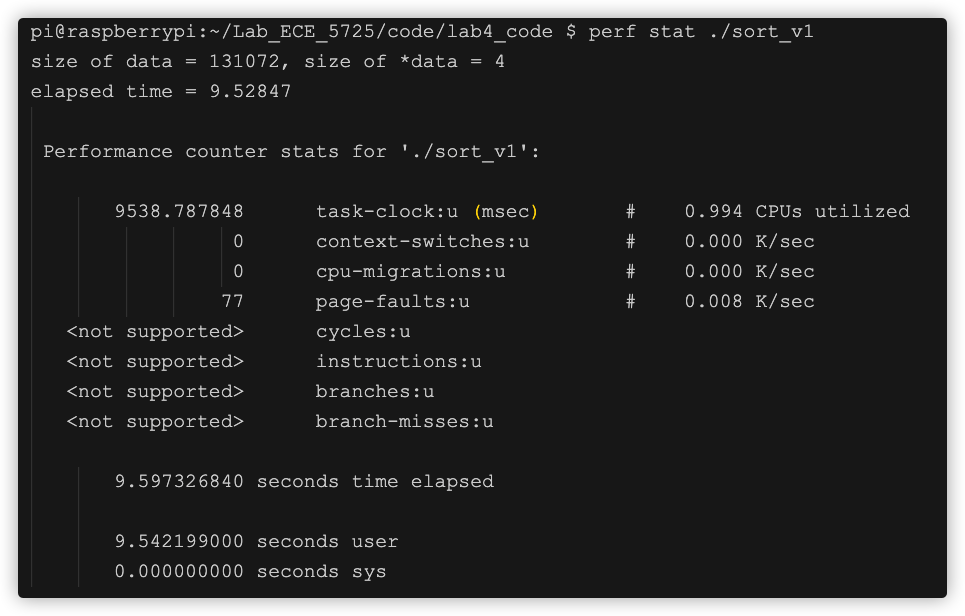
\includegraphics[width=\linewidth]{Images/unsortversion.png}
  \caption{Unsorted version on Preempt Kernel}
\end{minipage}%
\begin{minipage}{0.5\textwidth}
  \centering
  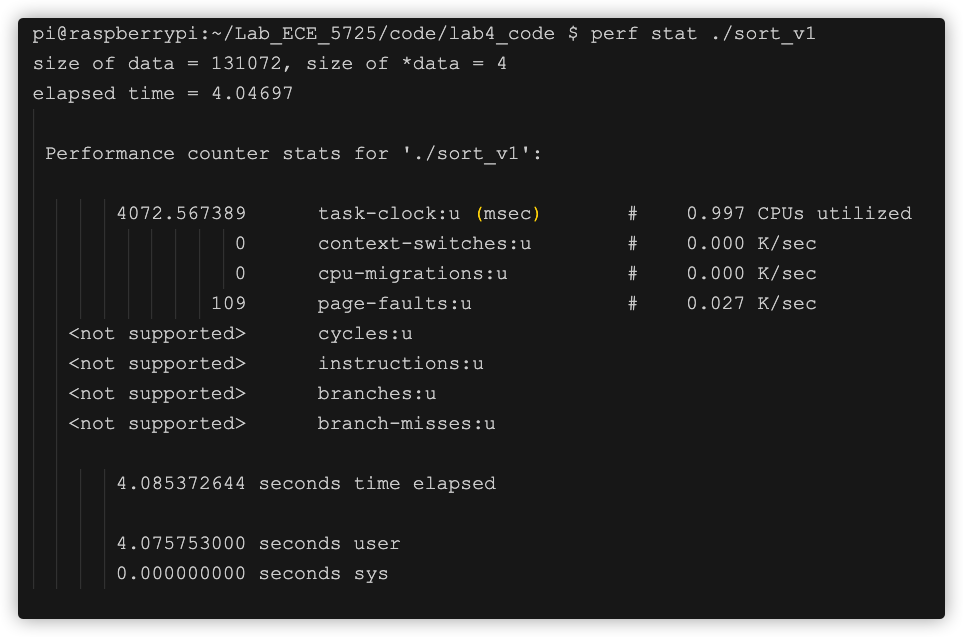
\includegraphics[width=\linewidth]{Images/sortversion.png}
  \caption{Sorted version on Preempt Kernel}
\end{minipage}
\end{figure}
We did not notice any significance difference between this result and the original kernel. The elapsed time is very similar ( about 4 seconds and about 9.6 seconds). The CPU's utilized only decreased by 0.006 - a fairly trivial amount. The page faults were also of similarly low numbers of the same magnitude. Since perf was unable to output the complete results on this kernel, it is possible that there are differences in cycles, instructions, branches, or branches missed - we just cannot speak to this. When considering the information given, there does not appear to be a significant difference between the original and PreemptRT kernel.



\textbf{Step 3: Square Wave Tests}

To perform the square wave test, we first needed to finish the skeleton code. This was easier than expected and only involved two additional lines of code. The code is shown below:
\begin{center}
\begin{lstlisting}[language=C, label=code:code16] 
while (1)
        {

                for (i = 0; i < interval; ++i)
                {       /// use delay loop to control frequency
                        // interval 1200 = about 60k Hz
                }

                //  code to control GPIO goes here....
                gpioWrite(26, PinValue);
                PinValue = PinValue ^ 1;
        }
\end{lstlisting}
\end{center}\vspace{-1em}
In the while loop, we use a for loop for implementing the time interval and then change the output of the GPIO pin 26 after every interval to realize the PWM output. After completing this code, we named it \code{test\_rt\_v16.c} and began a series of frequency test experiments. Rather than adjusting the frequency, we adjusted an arbitrary value (interval) and determined the output frequency from the scope. 

When running \code{test\_rt\_v16.c}, the frequency response increased as we decreased the interval. To estimate the maximum allowed frequency, we removed the for loop from the code. This resulted in very similar values (4.4\% difference), with 3.90MHz for the loaded system and 4.08MHz for the unloaded system. We obtained these results by averaging 5 readings, since they were fluctuating quite a bit. This difference might be due to poor readings. The maximum is considerably larger than what was achieved by the blink\_v7.c code in week 1 (50kHz). Unlike for the blink codes in C and in Python, there is no performance 'knee' as a upper frequency bound. Rather, the maximum frequency depends on the architecture (ex: limit of the scope or other hardware).  

\begin{figure}[H]
\centering
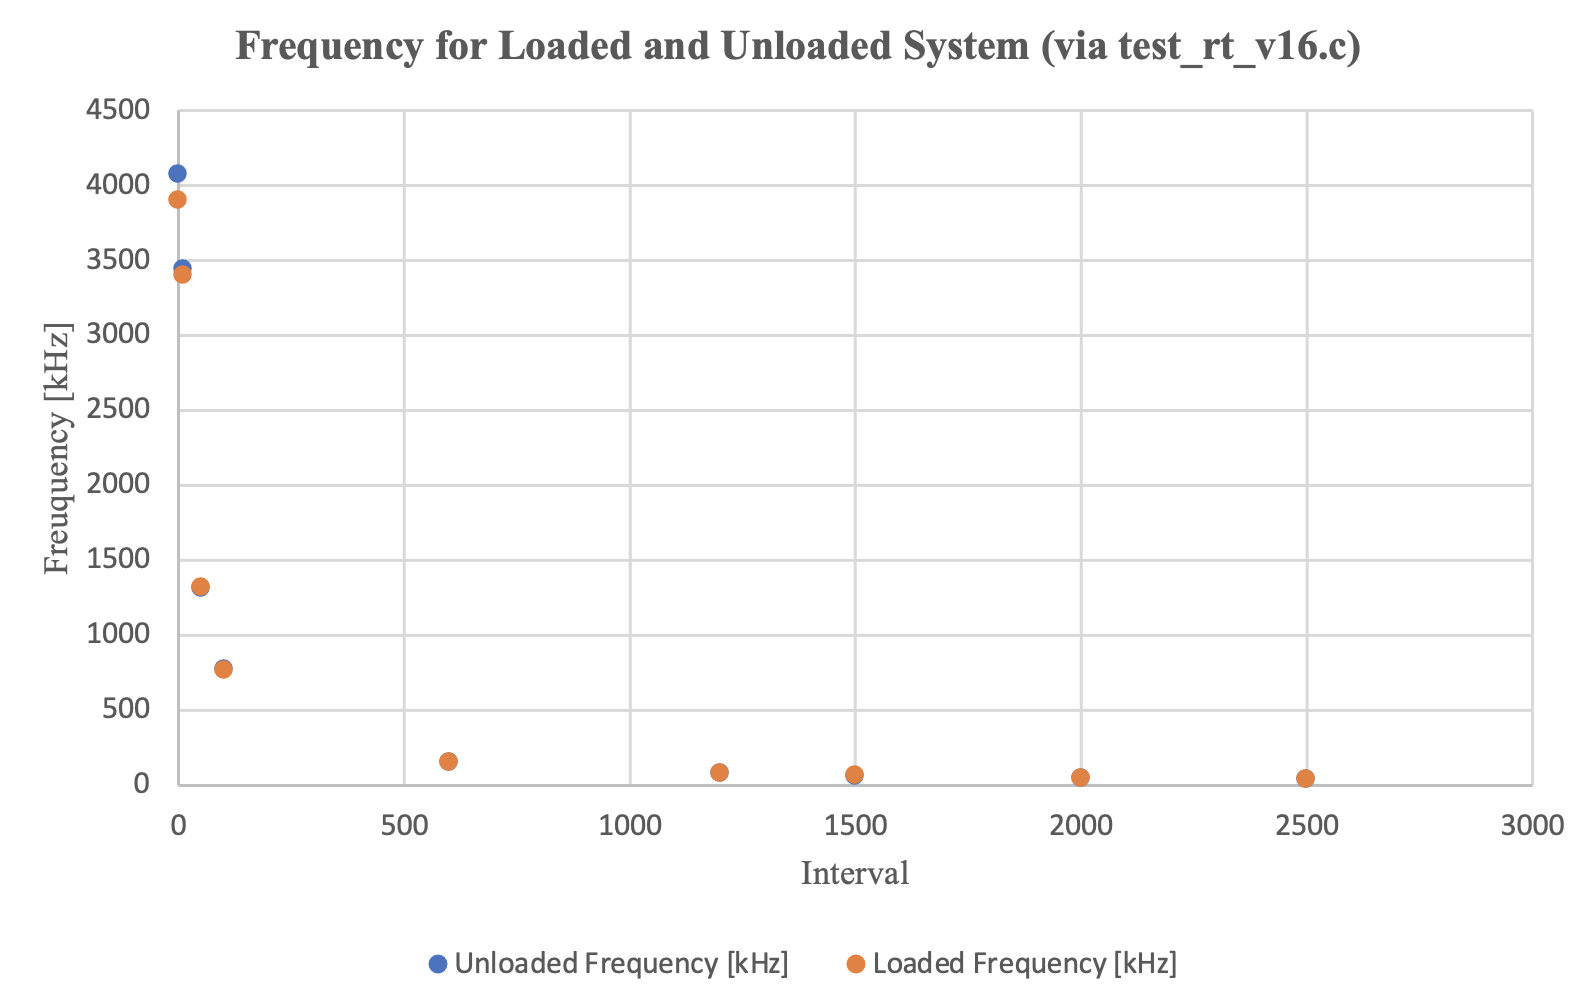
\includegraphics[width=0.75\linewidth]{Images/test_rt freq.png}
\caption{Frequency response for loaded and unloaded system}
\end{figure}

During the test, we used the command \code{ps -alef | grep test\_rt\_v16} to get the process ID of the \code{test\_rt\_v16.c} when the system is loading and unloading. Then we used the command \code{chrt -p pid} to get the real-time scheduling attributes of the \code{test\_rt\_v16.c}. We did the same for \code{blink.py}. Their \code{chrt} results are shown in the below figure:

\begin{figure}[H]
\centering
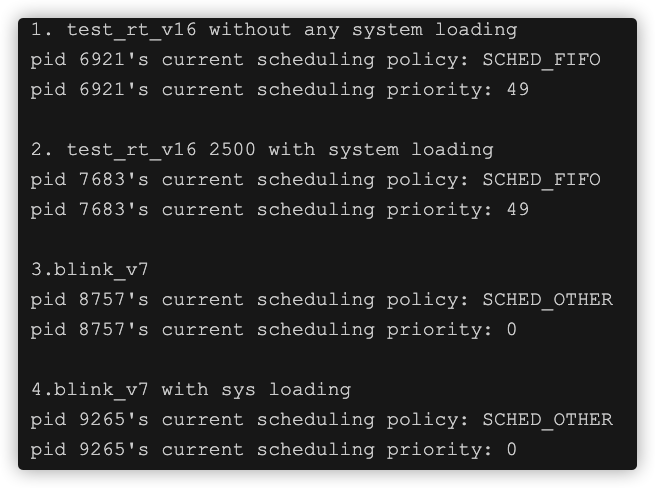
\includegraphics[width=0.4\linewidth]{Images/chrt.png}
\caption{Frequency response for loaded and unloaded system}
\label{fig:figure14}
\end{figure}
From the figure \ref{fig:figure14}, we can see that the scheduling policy for the \code{test\_rt\_v16} is \code{SCHED\_FIFO} which is a real-time policy and the priority of the \code{test\_rt\_v16} is 49 as we set in the code. Where priorities range from 1-99 and a higher value indicates a higher priority, realtime threads are given higher priority to ensure completion before the deadline. One drawback is when under high CPU load and set to real-time, the processor will be occupied until the process is finished and will not allow any other processes to run in parallel. 

On the other hand, we can find that the the scheduling policy for the \code{blink.py} is \code{SCHED\_OTHER}, which is a common round-robin time-sharing scheduling policy with a priority of the \code{blink.py} is 0. This schedules a process for a time-slot based on other tasks running on the system. Since the \code{blink.py} doesn't use a real-time strategy, its measured frequency with and without loading does not change. We were able to check out in lab on Monday.
 
\section{Conclusion}

Overall, this lab was straightforward and we were able to finish by the end of lab in both weeks. This lab strengthened our knowledge of the linux system and kernel configuration. It also showed the differences between non-real time and real-time systems through a series of performance tests, as well as demonstrated how the real-time system can  push a hardware system to its performance limits.

Real-time systems allow for more predictable process scheduling by increasing the speed of task management, allowing critical tasks to finish within their given deadlines, and reducing downtime. The effects were most clear in the result of C program. The maximum frequency of the C program is already very high in the original kernel but still limited by the system load. In the PreemptRT kernel, the maximum frequency of the C program has no limitation by other processes, rather its limitation is the architecture.

We were surprised by the results of the Python blink script in week 1, as we thought the unloaded system would outperform the loaded system. The results were due to noise introduced by Python, although it was unexpected for the noise to be large enough to noticeably impact the results.

The lab guidelines were clear, thorough, and easy to follow. Although mentioned in class, a brief note on finding the maximum allowed frequency in \code{test\_rt\_v6.c} (remove for loop) and finding the upper bound in \code{blink.py} and \code{blink_v7.c} (set to very large value first) might be helpful. 


\newpage
\section{Appendix}

\subsection{References}


[1] \textbf{Lab 4 Instructions:} https://canvas.cornell.edu/courses/32456/files/4556244?module\_item\_id=1204235

\subsection{Migrating System to a Larger SD Card}

https://peppe8o.com/raspberry-pi-migrating-to-larger-sd-card-with-windows-step-by-step-guide/


\end{document}